\documentclass[a4paper,12pt]{article}
\usepackage[T1]{fontenc}
\usepackage[latin9]{inputenc}
\usepackage{listings}
\usepackage{amsmath}
\usepackage{mathtools}
\usepackage{mathpazo}
\usepackage{wasysym}
\usepackage{graphicx}
\usepackage{tikz,pgfplots}
\usepackage[colorinlistoftodos]{todonotes}
\usepackage{natbib} 
\usepackage{geometry}
\usetikzlibrary{fit,shapes.misc,snakes}
\geometry{verbose,tmargin=2.5cm,bmargin=2.5cm,lmargin=2.5cm,rmargin=2.5cm}

\newcommand{\ord}{\operatorname{ord}}

\graphicspath{ {../Project1/measurements/final/} }

\begin{document}

\title{IO\\Project 1}

\author{Lasse Espeholt - 20093223\\
Kasper Nielsen - 20091182\\}

\maketitle
\begin{figure}[h!]
\includegraphics[width=\textwidth]{"images/forside"}
\end{figure}


\vfill{}
\begin{description}
\item [{Implementation~code~and~test~results:}]
\texttt{http://github.com/kasper0406/IO13/}
\end{description}
\pagebreak{}\tableofcontents{}\pagebreak{}

\section{Introduction}
This report describes the implementation of an external Mergesort and analyses the performance characteristics of the implemented streams and sorting algorithms, as outlined in the project description.


\section{Setup}
This section presents the test setup, how measurements are performed
and gives an overview of the files attached to this report.

\subsection{Test setup}
%!TEX root = rapport.tex
All measurements presented in this report were performed on a computer
with an Intel Core i3-380UM CPU with the following technical
specifications:
\begin{itemize}
\item 2 cores w/HT operating at 1.33GHz
\item 2 x 32KB L1 data cache
\item 2 x 256 KB L2 cache
\item Shared 3MB L3 cache
\end{itemize}
The main memory size of the machine was 1 GB (with approximately 600MB free memory), and the machine was running Ubuntu
Linux 12.04. The hard drive was an USB2 attached Fujitsu MJA2250BH which has the following specifications:

\begin{itemize}
\item 250GB
\item 5,400 RPM
\item 8MB cache
\item 512B sector size
\end{itemize}

The file system had a block size of 4096B and 128kB read ahead.

All implementations have been
written in C++11 and compiled on Linux using the GCC 4.7 compiler. When measurements were performed, the
code was compiled using the \texttt{-O3 -flto -funroll-loops}
optimization flags.

The variations between several runs were insignificant so we choose to run all tests once to be able to run as many configurations as possible.

\subsection{File structure}
The following is a description of the different folders handed in with
the report.
\begin{description}
\item[code] Contains the implementations of the different streams and
  the external memory sort.

\item[output] Contains the raw measurements used for the plots in the
  report. The plots themselves are also included in a pdf-format.
\end{description}

\subsubsection{Code structure}
The code has the following source files.
\begin{description}
\item[main.cpp] Driver code for calling test code.
\item[test.h] Test framework for testing streams and sorting with
  different parameters.
\item[utils.h] Responsible for generating large files for testing.
\item[CMakeLists.txt] CMake file for the project specifying
  compilation options.

\item[rw\_stream.h] Shared code for streams using \texttt{write} and
  \texttt{read} system calls. The unbuffered streams are implemented
  in:
  \begin{itemize}
  \item read\_input\_stream.h
  \item write\_output\_stream.h
  \end{itemize}
  The buffered streams are implemented in:
  \begin{itemize}
  \item buffered\_input\_stream.h
  \item buffered\_output\_stream.h
  \end{itemize}

\item[f\_stream.h] Shared code for streams using \texttt{fwrite} and
  \texttt{fread} functions from the C standard library. Specific
  stream implementations are:
  \begin{itemize}
  \item fread\_input\_stream.h
  \item fwrite\_output\_stream.h
  \end{itemize}

\item[mmap\_stream.h] Shared code for streams using memory mapping of
  files. Specific stream implementations are:
  \begin{itemize}
  \item mmap\_input\_stream.h
  \item mmap\_output\_stream.h
  \end{itemize}
\end{description}

\section{Streams}
This section presents how benchmarks of the four different
streams were performed, and an analysis of their performance. First each stream will
be treated separately and the best settings for each stream will be
used in a relative performance benchmark for finding the stream most
suitable for sorting.

In order to mimic the behaviour of sorting during the test, we have
tested the streams in respectively reading/writing $N$ elements from/to a file. Each test uses $k$ interleaved streams, such
that a new stream is starting at every $\frac{N}{k}$ elements, and
elements are being processed in a round robin fashion of the streams.

All tests of the streams have used $N = 2^{28}$, which corresponds to
1GB of elements. This choice was made to make sure the data could not be hold in memory in its entirety, and still small enough to be able to run all the tests within reasonably time. The
number of elements has not been varied for the stream test, as it is not
expected that streams will behave differently, as long as the data is
big enough to not fit the main memory.

In the merge step in the sorting application, the input streams are
used in a very similar way, the output streams are however only used
in the $k = 1$ case, but we have chosen to do testing of these streams
for varying values of $k$, to be able to get comparable results
between input and output streams.

\subsection{Buffered streams}
\label{sec:buffered-streams}
This type of streams are implemented using the \texttt{read} and
\texttt{write} POSIX system calls. On top of those, a buffer of size
$B$ is added such that the system calls are only called once for $B$ elements. This section investigates how the choice of buffer size and varying
values of $k$ influences the
performance.

Figure~\ref{fig:buffered-input} shows a plot of the performance for the buffered input stream.

\begin{figure}[h!]
  \centering
  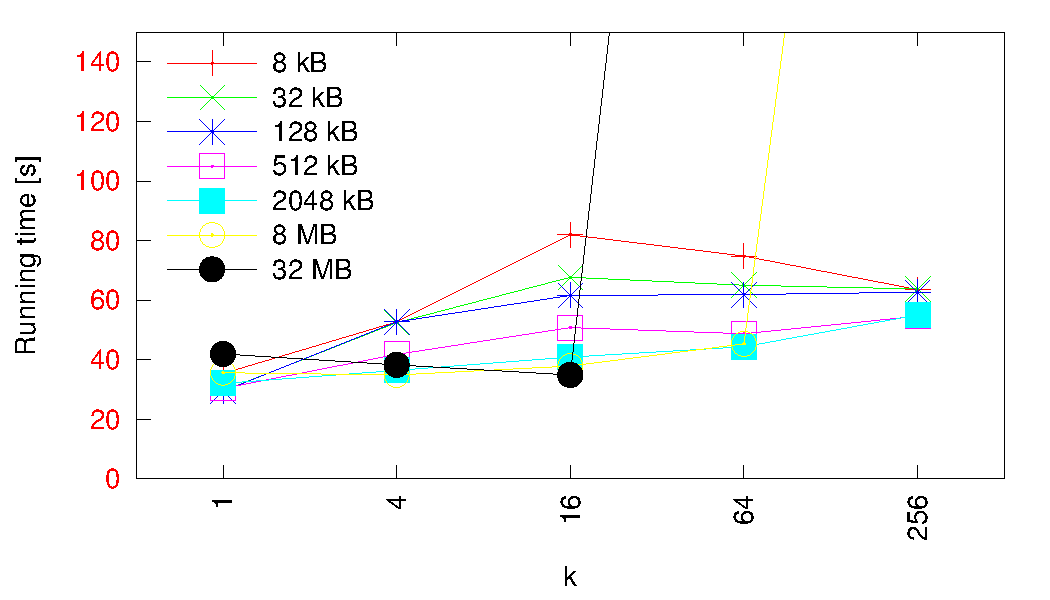
\includegraphics[width=0.8\textwidth]{buffered_input}
  \caption{Running times for the buffered input stream using different
    buffer sizes and varying $k$-values.}
  \label{fig:buffered-input}
\end{figure}

From Figure~\ref{fig:buffered-input} it seems like all the streams
perform similarly for sequential read ($k = 1$). This is most likely because the operation system and the disk controller easily can classify the access pattern as sequential and hence, can cache the subsequent blocks with very low cost.

As $k$ gets bigger, Figure~\ref{fig:buffered-input} indicates that
bigger buffers gives better performance, which was expected. However,
for large buffer sizes in combination with large values of $k$, the
input stream performs extremely poorly. The decrease in performance happens because the
buffers partly ends up on disk because of insufficient free memory causing memory thrashing. Experiments with larger buffer sizes were also performed and they
showed a similar behaviour and are therefore of no
interest for use in sorting.


Figure~\ref{fig:buffered-input} shows a small curve for smaller buffer sizes. We speculate that...
\todo{data ligger langt fra hinanden vs. den kan lave readahead + data begynder at ligge taet + cache paa disk. Hhm hvordan kan det passe for 8kB? Jo tror det er fint det argument med cache}

From Figure~\ref{fig:buffered-input}, it seems that a buffer size of 2
MB provides the best compromise of running time and memory usage for
the input stream in the sorting application.

For the output stream a similar plot is shown in
Figure~\ref{fig:buffered-output}.

\begin{figure}[h!]
  \centering
  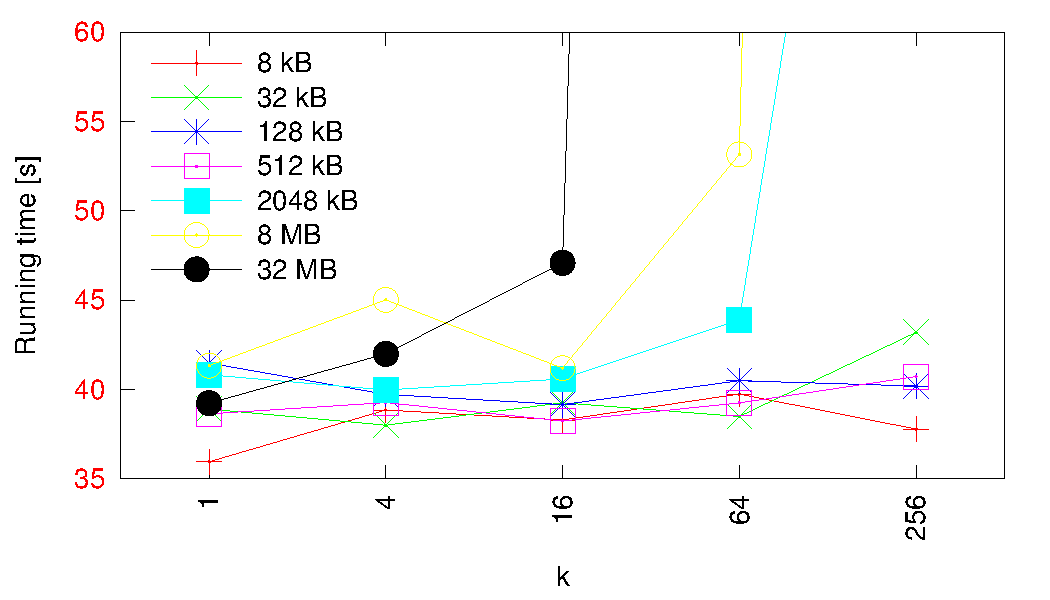
\includegraphics[width=0.8\textwidth]{buffered_output}
  \caption{Running times for the buffered output stream using different
    buffer sizes and varying $k$-values.}
  \label{fig:buffered-output}
\end{figure}

We expected that the plots in Figure~\ref{fig:buffered-input} and
Figure~\ref{fig:buffered-output} would be similar since the two streams
are much alike. However, the plots shows that the varying the buffer sizes
almost have no effect on the performance of the output streams (except
when they are too big to be in memory.)\todo{This seems to happen before
  in the write case?}

The disk controller has the choice of delaying writes to the disk platters by using its 8MB cache and wait until it receives more data in the same region of the disk. It thereby avoids random seeks. This could explain why varying buffer sizes performs equally.

An experiment was performed, where the
\texttt{fsync(2)}\footnote{The \texttt{fsync(2)} system call ensures
  that the file is written to disk immediately.} system call was
called immediately after each write operation. It was found that both
the input and output streams performed very similar, hence the absence
of effect in varying buffer sizes showed in
Figure~\ref{fig:buffered-output} can be explained by the write cache of the disk.

A buffer size of 2 MB has been chosen to give the best trade-off
between running time and memory consumption. From
Figure~\ref{fig:buffered-output} it seems like a tiny buffer would be
a better choice but for external Mergesort only $k=1$ is used. Therefore, we choose to base our choice on the performance of the input streams.

\subsection{MMap streams}
For the memory mapped streams, the \texttt{mmap} and \texttt{munmap}
system calls are used for mapping a file into memory. Then the file
can be accessed as it was loaded into memory, but the actual loading
is lazy, such that it only happens when it is needed.

Therefore it is expected that the block size mapped into memory each
time \texttt{mmap} is called, will not have any significant impact on
the results, since only some memory bookkeeping and different amount
of remapping is required when using different block sizes. This
however, should be negligible compared to the time of the actual disk
access.

\begin{figure}[h!]
  \centering
  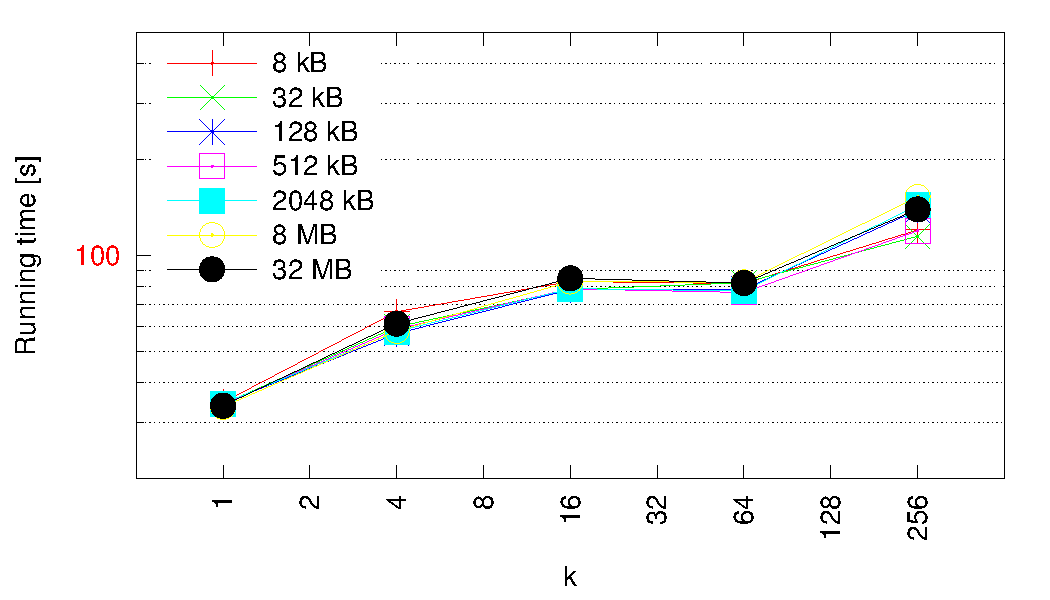
\includegraphics[width=0.8\textwidth]{mmap_input}
  \caption{Running times for the mmap input stream, varying sizes of
    mapped blocks and $k$-values.}
  \label{fig:mmap-input}
\end{figure}

Figure~\ref{fig:mmap-input} shows a plot of the running times for the
mmapped input stream. Except for the case $k = 256$, the plot shows
that the running times for the different block sizes are very close,
which is expected. For the $k = 256$ case, it seems like some choices
of block sizes are better than others, but there does not seem to be an
obvious correlation on how the block sizes influences the running time
in this case. This may simply be because of variance in the
measurements.

The running time of input stream was found to be worse when the value
of $k$ was increased. We speculate that the performance decrease is caused by the operating system's bookkeeping. Normally, one would not use different mappings in the same process but only a single one where each stream would get a pointer to different memory locations.\todo{Et andet argument kunne vaere at det bliver mere tilfaeldigt hvad der bliver laest naeste gang}

\begin{figure}[h!]
  \centering
  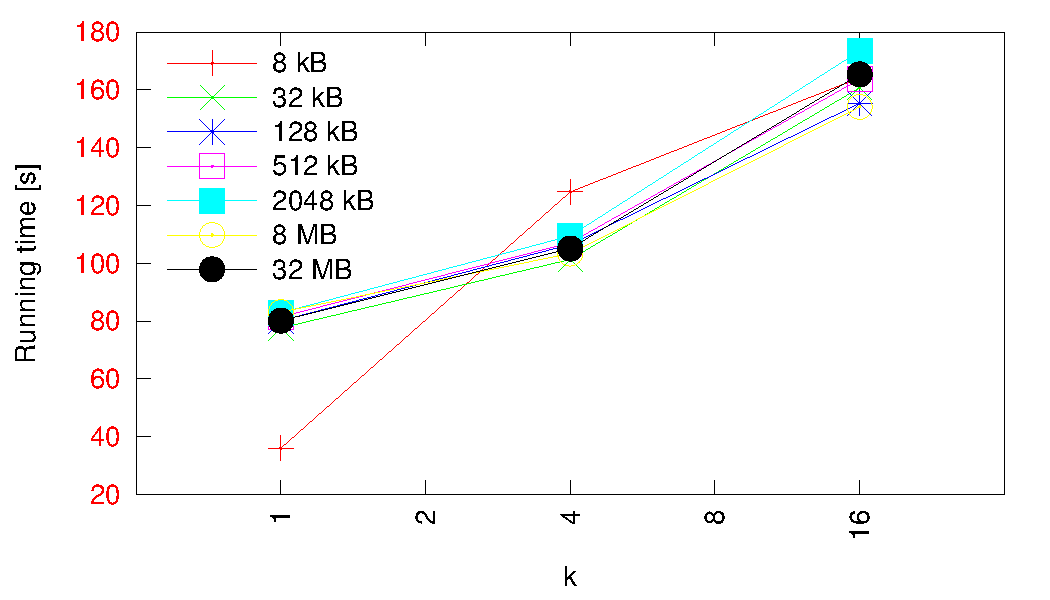
\includegraphics[width=0.8\textwidth]{mmap_output}
  \caption{Running times for the mmap output stream, varying sizes of
    mapped blocks and $k$-values.}
  \label{fig:mmap-output}
\end{figure}

A similar plot for the mmap output stream is shown at
Figure~\ref{fig:mmap-output}. For the output stream it seems like the
different streams behaves alike for different buffer sizes, except
when the block size is 8kB. The 8kB block performs substantially
better when $k = 1$, but worse when $k = 4$\todo{Why? Jeg har nye plots, lad os kigge paa dem}.

Like the input stream, the performance of the output stream is
decreasing for larger values of $k$, and no test with $k$ greater than
16 was performed due to long execution times.

\subsection{Other streams}
\label{sec:other-streams}
This section will discuss the two remaining stream
implementations. The first of these are the streams using the
\texttt{fwrite} and \texttt{fread} C standard library calls, which
themselves do buffering. At our test machine the default buffer size
of \texttt{fread} and \texttt{fwrite} was 8
kB. Figure~\ref{fig:fstreams} shows a plot of their performance.

\begin{figure}[h!]
  \centering
  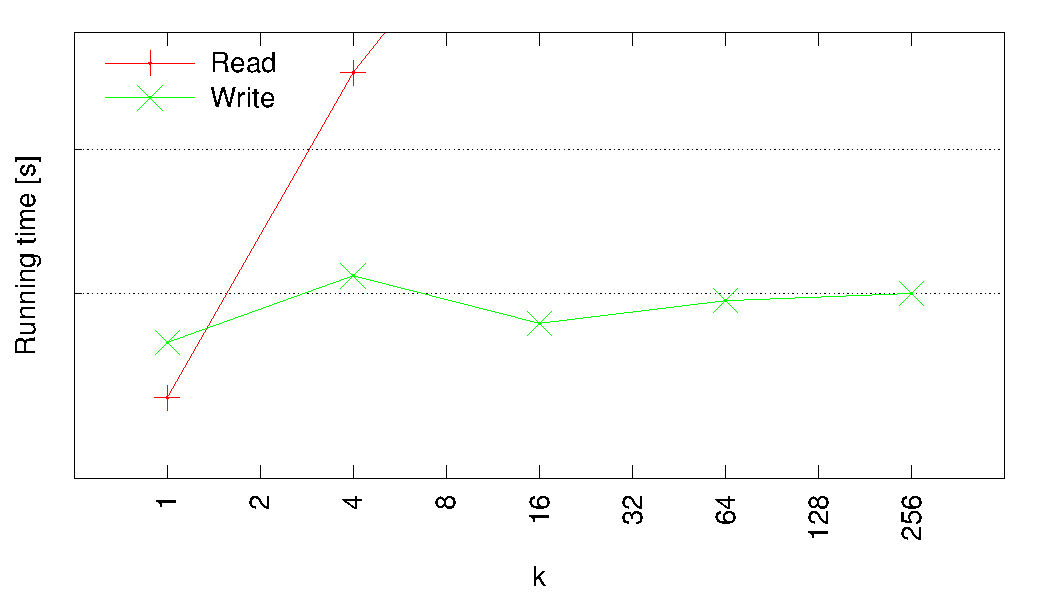
\includegraphics[width=0.8\textwidth]{fstreams}
  \caption{Running times for the streams using the \texttt{fwrite} and
    \texttt{fread} standard library functions, varying the values of
    $k$.}
  \label{fig:fstreams}
\end{figure}

Comparing Figure~\ref{fig:fstreams} to our buffered streams, they show
a very similar behaviour. This is as expected, since the streams
should function in exactly the same way.

We will now turn our attention to the streams using the \texttt{read}
and \texttt{write} system calls directly. Due to extremely poor
performance, only one measurement for the output stream was
obtained. The results are plotted in Figure~\ref{fig:syscall-streams}.

\begin{figure}[h!]
  \centering
  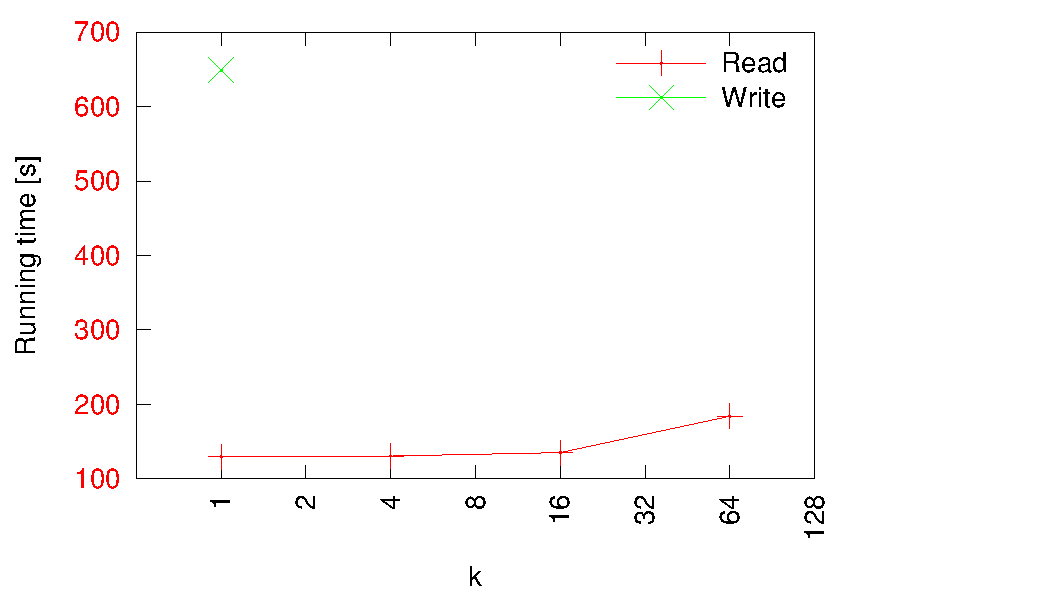
\includegraphics[width=0.8\textwidth]{syscall_streams}
  \caption{Running times for the streams using the \texttt{write} and
    \texttt{read} system calls directly, varying the values of $k$.}
  \label{fig:syscall-streams}
\end{figure}

The input stream has an almost constant running time from $k$ between
1 and 16. However, for $k = 64$ a small increase in running time is
seen, which ...\todo{Describe why? naar vi kommer tilbage til foerste stream, er alt ude af cachen pga readahead*64>8MB cache}.

As mentioned earlier, only one measurement was done for the output
stream. It is a bit surprising that the output stream is so much
slower than the input stream. The the smallest unit able to be written
to the disk is a sector, which on the test machine is
512B. If smaller amount should be written, it is\todo{Probably BS}
required that the sector is read, modified in memory and then written
back to the disk. When the \texttt{write} system call is used without
buffering, this happens every time an integer is written to the
stream, causing a tremendous overhead, resulting in the extremely
large running time.

\subsection{Relative comparison}
In order to determine which stream to use, it is very important that
the input streams performs well for varying values of $k$. This
however, is not as important for the output stream since it is not
interleaved, but other disk access may happen in between writes to the
output stream in the sorting, meaning that it is also is preferable if
the output stream performs decently for different $k$ values, as this
indicate that the output stream is more robust for interleaved disk
operations.

In order to chose which stream to use in sorting, we have picked out
the input and output streams from the previous sections, which had the
best performance across all values of $k$. In this section we will
compare them, and single out a winner for use in sorting.

Figure~\ref{fig:best-input} shows the running times for what was found
to be the best input streams. This plot suggests that the buffered
input stream with 2MB buffer is the best choice, whereby we have
chosen to use this for sorting.

\begin{figure}[h!]
  \centering
  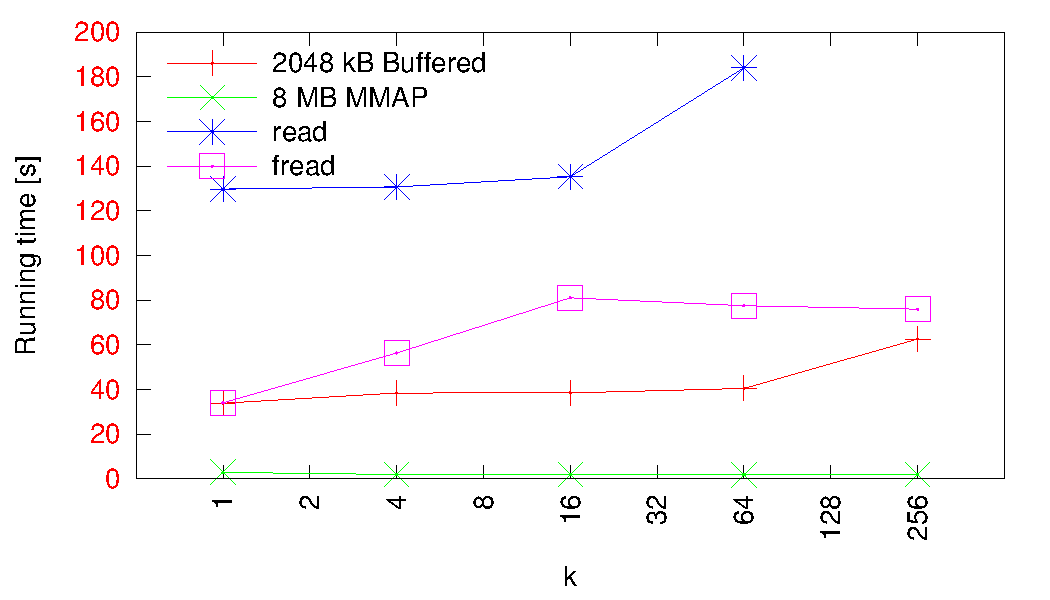
\includegraphics[width=0.8\textwidth]{best_input}
  \caption{Comparison of the best input streams from each of the four
    types of streams.}
  \label{fig:best-input}
\end{figure}

Figure~\ref{fig:best-output} shows a plot of the best output
streams. The only real competition is between the \texttt{fwrite} and
the buffered output stream with 2MB buffer. As discussed in
Section~\ref{sec:other-streams} the streams are functioning in almost
the same way, except they use a different buffer size. From the extra
experiment performed in Section~\ref{sec:buffered-streams}, it was
found that a small buffer was significantly worse if data was forced
to be written to the disk instantly after the buffer is full. This is
the case for sorting, since the operations in the next iteration
relies on these data. Therefore we have chosen to use the buffered
output stream with a 2MB buffer, even though
Figure~\ref{fig:best-output} seems to suggest it is performing
slightly worse at $k = 256$\todo{Do another plot justifying this? Nope, slet det med write, fokuser paa read}.

\begin{figure}[h!]
  \centering
  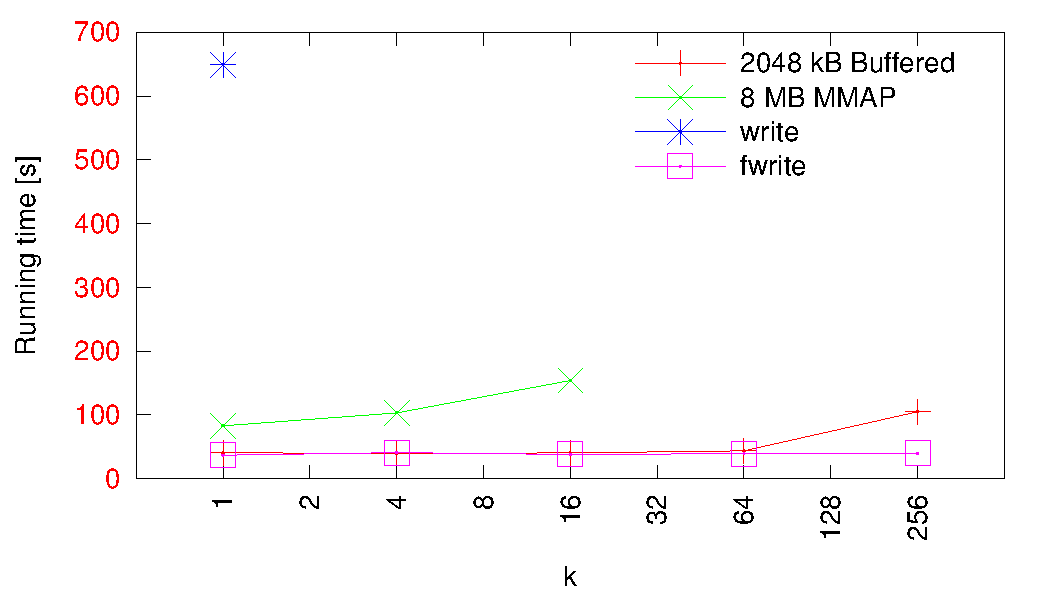
\includegraphics[width=0.8\textwidth]{best_output}
  \caption{Comparison of the best output streams from each of the four
    types of streams.}
  \label{fig:best-output}
\end{figure}

\section{Sorting}
This section will investigate how the external memory merge sort
performs for different choices of parameters. Given the input size
$N$, the algorithm has two parameters to tweak: The memory size $M$,
and the number, $k$, of input streams to merge simultaneously.

There are some constraints on these parameters. It will not make sense
to have $M$ bigger than the actual memory size, since this corresponds
to a conventional in-memory sorting. Similarly it must be that $k <
\frac{N}{M}$, since there should be at least $k$ streams to merge.

Figure~\ref{fig:sorting} plots the running time of sorting 1GB of
integers, using different settings for the $M$ and $k$ values. It is
seen, that the measurements seems to form around the same levels of
running times when varying the parameters. This is due to the number
of times the file is read on the disk.

For every level in the merge tree, the file is read and written once
from/to the disk. The height of the merge tree for give parameters is
$h = \log_k \frac{N}{M}$, since every merge merges $k$ streams, and
there are $\frac{N}{M}$ streams initially. The levels seen in
Figure~\ref{fig:sorting} follows this bound very nicely.

There are small variations for the running time of each level, but
these seems almost negligible in the overall picture. This also
suggests that the assumption of the I/O model, where only disk
accesses are the thing to count, indeed seems to be a good model in
practice when the input does not fit into main memory.

For a given choice of parameters, the amount of memory used to sort
the file is given by $M + B\frac{N}{M}$. Hence, the different
measurements with the same height, use a different amount of
memory. This gives another criteria to optimize when choosing
parameters: First the height of the merge tree should be minimized,
then the amount of used memory. There will be some cases where the
minimum height merge tree is not the best thing to choose, since the
parameters obtaining this will not fit the memory of the machine. This
is seen for $M = 2$ and $k \geq 256$ in Figure~\ref{fig:sorting}.

When sorting 1GB of integers, we have found parameters $M = 32MB, k =
32$ and $M = 64, k = 64$ to be the ones using less memory, both using $96MB$.

\begin{figure}[h!]
  \centering
  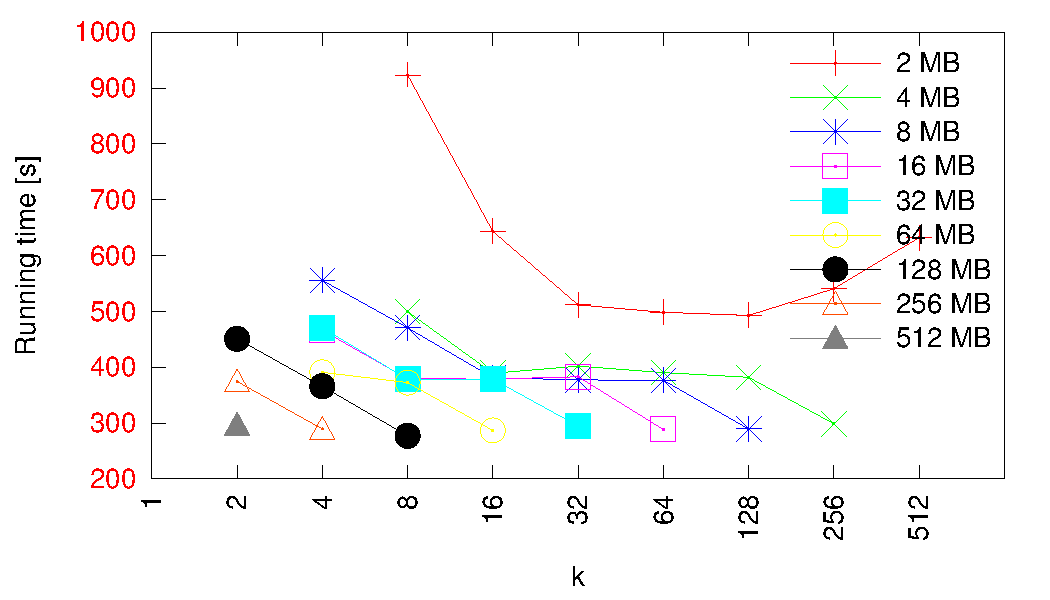
\includegraphics[width=0.8\textwidth]{sorting2}
  \caption{Time for sorting a 1GB file varying the memory size $M$ and
    streams to merge in parallel $k$.}
  \label{fig:sorting}
\end{figure}

\subsection{Comparison with conventional sorting algorithms}
In order to determine how well the external merge sort is performing,
it has been benchmarked against conventional quick sort and heap sort
implementations. The quick sort is from the C standard library, and
the heap sort is from STL. A plot of the running time for the
different sorting algorithms is shown in Figure~\ref{fig:best-sort}.

\begin{figure}[h!]
  \centering
  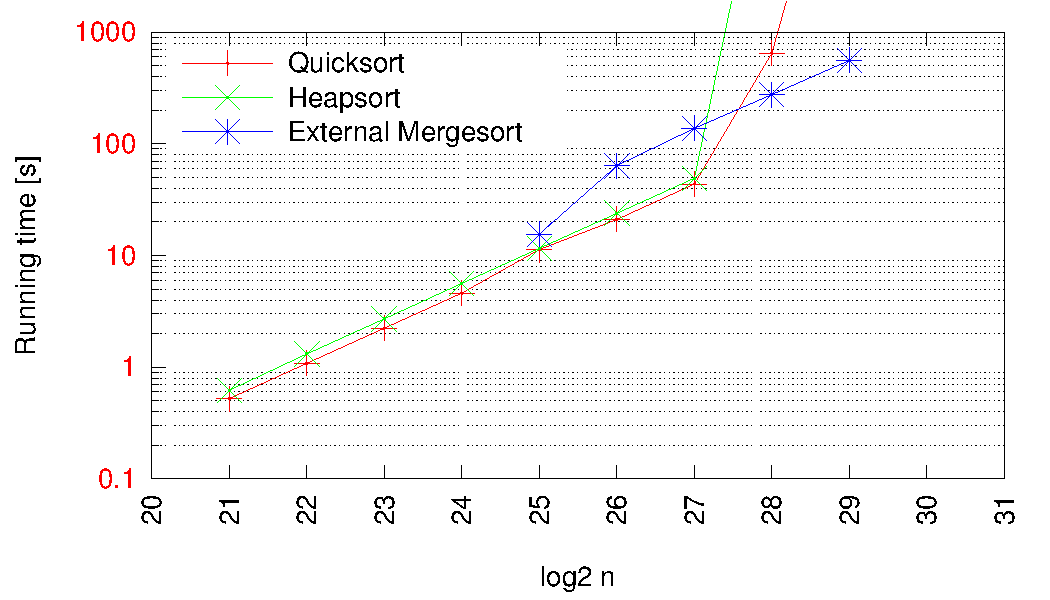
\includegraphics[width=0.8\textwidth]{best_sort}
  \caption{Comparison of the different sorting algorithms varying the input size.}
  \label{fig:best-sort}
\end{figure}

It can be seen that both quick sort and heap sort outperforms the
external merge sort when $n \leq 2^{27}$, which is 512MB of
elements. This is no surprise, since both quick and heap sort are
in-place sorts. The test machine was equipped with 1GB memory, hence
the two sorting algorithms can do everything without going to disk,
while the external merge sort by construction have to do merging on
the disk.

The other thing to notice, is that as soon as the input does not fit
the memory anymore $n \geq 2^{28}$ (1GB of elements), the external
merge sort beats the quick and heap sorts hands down. This was also
what we expected, wince the external merge sort should use the disk
much more efficiently.

\section{Conclusion}
In the course of the project, four different stream implementations
have been made and tested with an eye to the application of external
merge sort. It was possible to single out a winner among the
implemented streams, which was found it to be buffered streams with
2MB of buffer size.

It was found that the implemented external Mergesort tremendously improved the
performance of sorting large input, compared to conventional main
memory sorting algorithms -- for sorting 1GB of integer elements, we
found a performance increase of a factor\todo{insert impressive
  factor. + ~algoritme + ved 2GB var heap/qsort absurd langsomt}.

The overall findings of this project was therefore in agreement with
what should be expected from the I/O-model for analyzing algorithms.
\todo{meget vigtigt med hoejden af traeet (i.e. antallet af I/O)}

\clearpage{}\bibliographystyle{plain}
\addcontentsline{toc}{section}{\refname}\bibliography{ref}

\end{document}
